% Chapter Design

\chapter{Design}

\label{Chapter:Design}

A detailed description of the sharding protocol design with Bazo as the underlying blockchain is covered in this chapter.

\section{System Setting and Assumptions}

This section outlines the system setting provided by the current state of the Bazo blockchain and makes assumptions about the future state that is desired at the end.

\subsection{Entities}

Bazo consists of four entities: \textit{users}, \textit{validators}, \textit{leaders} and \textit{aggregators}. A \textit{user} is an entity who uses Bazo's infrastructure to transfer funds or run smart contracts. A \textit{validator} is a node in the network who participates in Bazo's consensus protocol and validates blocks. While users only store block headers, validators store block headers and bodies of their assigned shard. For the sake of simplicity, examples in this paper assume that every user is a validator.

Furthermore, there are two special types of validators: A \textit{leader} is a validator who has the right to append the next block to the blockchain of one particular shard. An \textit{aggregator} is a validator who is responsible for the aggregation of transactions to reduce the overall size of the blockchain. 

Each entity of the network has a public-private key-pair to digitally sign transactions. Bazo employs elliptic curve digital signature algorithm (ECDSA) as the base signing algorithm. In the rest of this paper, we refer to this ECDSA key-pair as to the user's \textit{wallet keys} $(pk_{wall}, sk_{wall})$.
\begin{figure}[hbt]
  \centering
  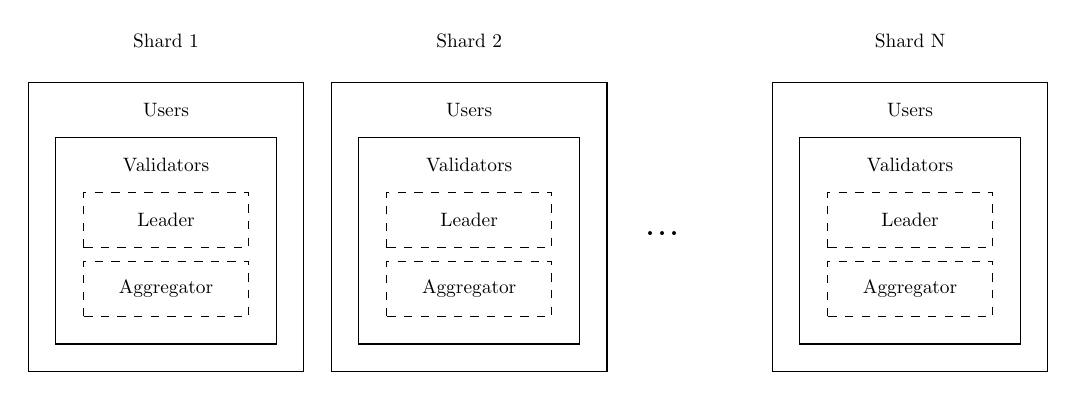
\begin{tikzpicture}[scale=0.7, every node/.style={transform shape}]
  
  %\draw[step=1cm,gray,very thin] (0,0) grid (20,7);
  
  % ***************** SHARD 1 ***************** 
  \node at (2.5,6) {Shard 1};
  
  \draw (0,0) rectangle (5,5.25);
  \node at (2.5,4.75) {Users};
  
  \draw (0.5,0.5) rectangle (4.5,4.25);
  \node at (2.5,3.75) {Validators};
  
  \draw[dashed] (1,2.25) rectangle (4,3.25);
  \node at (2.5,2.75) {Leader};
  
  \draw[dashed] (1,1) rectangle (4,2);
  \node at (2.5,1.5) {Aggregator};
  
  % ***************** SHARD 2 ***************** 
  \node at (8,6) {Shard 2};
  
  \draw (5.5,0) rectangle (10.5,5.25);
  \node at (8,4.75) {Users};
  
  \draw (6,0.5) rectangle (10,4.25);
  \node at (8,3.75) {Validators};
  
  \draw[dashed] (6.5,2.25) rectangle (9.5,3.25);
  \node at (8,2.75) {Leader};
  
  \draw[dashed] (6.5,1) rectangle (9.5,2);
  \node at (8,1.5) {Aggregator};
  
  % ***************** DOTS ***************** 
  
  \node at (11.5,2.5) {\Huge{...}};
  
  % ***************** SHARD N ***************** 
  \node at (16,6) {Shard N};
  
  \draw (13.5,0) rectangle (18.5,5.25);
  \node at (16,4.75) {Users};
  
  \draw (14,0.5) rectangle (18,4.25);
  \node at (16,3.75) {Validators};
  
  \draw[dashed] (14.5,2.25) rectangle (17.5,3.25);
  \node at (16,2.75) {Leader};
  
  \draw[dashed] (14.5,1) rectangle (17.5,2);
  \node at (16,1.5) {Aggregator};
  
  \end{tikzpicture}
  \caption{An overview of entities in the Bazo blockchain.\label{fig:Entities}}
\end{figure}

Figure \ref{fig:Entities} shows that entities are equally partitioned into shards $1$ to $N$. While users and validators always remain in their particular shard based on their wallet address $pk_{wall}$, leaders and aggregators change block-wise. An aggregator is randomly elected in-shard and a validator is randomly elected cross-shard.

Furthermore, when a user wants to join the set of validators it must create an additional public-private key-pair using RSA and publish a stake transaction containing the public key. Note that this key-pair differs to the key-pair used to sign transactions. In the rest of this paper, we refer to this RSA key-pair as to the user's \textit{commitment keys} $(pk_{comm}, sk_{comm})$.

\subsection{Network Sharding}
\label{Design:NetworkSharding}

The Bazo infrastructure is divided into several subgroups referred to as \textit{shard}, each having it's own blockchain called \textit{shardchain}. Transactions of users are stored in a transaction pool by every validator in the network, but are only validated by validators based on the public wallet address $pk_{wall}$ of sender or receiver. For example, a validator $V$ of shard $S$ is responsible for user $U$ and validates transactions where $U$ is either sender or receiver of funds in a transaction. Thus, user $U$ is \textit{assigned} to shard $S$.

Likewise, validators are only responsible for the maintenance of the shardchain based on their $pk_{wall}$. Maintenance is hereby defined as validating blocks and storing the full shardchain. Responsibilities of leaders are outlined in Section \ref{Design:TransactionSharding}. 

Note that users also receive blocks but unlike validators, they do not participate in the validation process, which is further explained in Section \ref{Design:TransactionValidation}. Users in Bazo can be compared to SPV clients in Bitcoin, i.e., they only store their own transactions and block headers of the shardchain they belong to. To put it differently, validators store every block header received from the network, but only validate blocks based on their $pk_{wall}$.

\subsection{Epochs} 

The algorithm proceeds in \textit{epochs}. An epoch $e$ ends after a predefined number of blocks, that is, assume that epoch length $length_{ep} = 100$. Epoch $e$ starts at block number $1$ and ends after block number $100$, and the next epoch $e + 1$ starts at block number $101$ and ends after block number $200$, and so on. Furthermore, the process of ending an epoch is called \textit{finalization}. An epoch finalizes with a special type of block called \textit{epoch block}, denoted $eb$. An epoch block serves as a marker. Epoch finality is further explained in Section \ref{Design:Finality}.

\begin{figure}[hbt]
\centering
\captionsetup{justification=centering}
  \begin{tikzpicture}[scale=0.9, every node/.style={transform shape}]
      % Setup the style for the states
      \tikzset{node style/.style={state,minimum width=8mm,minimum height=8mm,rectangle}}
  
      \node[node style]                (eb1) {$eb^1$};
      
      \node[node style, right=of eb1] (sb22) {$sb_2^2$};
      \node[node style, above=of sb22] (sb12) {$sb_1^2$};
      \node[node style, below=of sb22] (sb32) {$sb_3^2$};
      
      \node[node style, right=of sb22] (sb23) {$sb_2^3$};
      \node[node style, above=of sb23] (sb13) {$sb_1^3$};
      \node[node style, below=of sb23] (sb33) {$sb_3^3$};
      
      \node[node style, right=of sb23] (sb24) {$sb_2^4$};
      \node[node style, above=of sb24] (sb14) {$sb_1^4$};
      \node[node style, below=of sb24] (sb34) {$sb_3^4$};
      
      \node[node style, right=of sb24] (eb5)   {$eb^5$};
      
      \node[node style, right=of eb5] (sb26) {$sb_2^6$};
      \node[node style, above=of sb26] (sb16) {$sb_1^6$};
      \node[node style, below=of sb26] (sb36) {$sb_3^6$};
      
      \node[draw=none,  right=of sb26]   (sb2dots) {$\cdots$};
      \node[draw=none,  right=of sb16]   (sb1dots) {$\cdots$};
      \node[draw=none,  right=of sb36]   (sb3dots) {$\cdots$};
  
  \draw[>=latex,
        auto=left,
        every loop]
       (sb12)   edge node {}   (eb1)
       (sb22)   edge node {}   (eb1)
       (sb32)   edge node {}   (eb1)
       
       (sb13)   edge node {}   (sb12)
       (sb23)   edge node {}   (sb22)
       (sb33)   edge node {}   (sb32)
       
       (sb14)   edge node {}   (sb13)
       (sb24)   edge node {}   (sb23)
       (sb34)   edge node {}   (sb33)
       
       (eb5)   edge node {}   (sb14)
       (eb5)   edge node {}   (sb24)
       (eb5)   edge node {}   (sb34)
       
       (sb16)   edge node {}   (eb5)
       (sb26)   edge node {}   (eb5)
       (sb36)   edge node {}   (eb5)
       
       (sb1dots)   edge node {}   (sb16)
       (sb2dots)   edge node {}   (sb26)
       (sb3dots)   edge node {}   (sb36); 
       
  \end{tikzpicture}
  \caption{The concept of epochs with number of shards $NofShards = 3$ and epoch length $length_{ep} = 3$.}
  \label{fig:shard_overview}
\end{figure}

An example is shown in Figure \ref{fig:shard_overview}. The Bazo blockchain starts with epoch block $eb^{h}$ and partitions the state into three shardchains $sb_{1-3}^h$, where $sb_{1-3}$ is a shard block of shardchain between one and three, and where $h$ is the block height. In this example, epoch length $length_{ep} = 3$. Thus, if three blocks have been created since the last epoch block, the current epoch is being finalized. Epoch block $eb^5$ is non-interactively created.

\subsection{Number of Shards}
\label{Design:NumberOfShards}

The number of shards is an important property that determines the overall scalability of the blockchain. As the number of transaction increases, the computational resources and network bandwidth required for processing transactions increases for each individual node. A balance between the number of users and the number of shards is crucial because
\begin{enumerate}
  \item having only one shard is equal to a blockchain without sharding, 
  \item having too few shards only scales sub-linearly as the number of users increases, or
  \item having too many shards increases the communication overhead required to synchronize the block height.
\end{enumerate}
Hence, a load-balancing algorithm is required to dynamically adjust the number of shards as new users are joining and using the network. 

As a first approach, the number of shards could be determined by the sum of all staked coins of the network divided by a predefined constant value that specifies the staking power per shard. This approach has the advantage that the number of shards increases (or decreases) in proportion to the actual staking power of the network. Unfortunately, the number of shards could easily be faked by a single user with a large amount of staked coins. 

A second approach would be to determine the number of shards by dividing the number of all validators of the network by a predefined constant value that specifies the number of validators per shard. This approach has the advantage that the number of shards increases (or decreases) in proportion to the actual number of validators of the network. However, the disadvantage of this approach is that the number of shards can easily be faked by a user with many wallets containing a few coins.

The last approach is to determine the number of shards by the Equation
\begin{gather}
\label{eq:NofShards}
  NofShards = \left\lceil \frac{NofUsers}{NofUsersPerShard} \right\rceil,
\end{gather}
where \textit{NofUsers} is the total amount users of the network, and where \textit{NofUsersPerShard} is a predefined value that specifies the number of users per shard. The second step is to verify if the number of shards is lower than the number of validators, i.e., 
\begin{gather}
\label{eq:NofShardsVerify}
  NofShards \geq NofValidators,
\end{gather}
where \textit{NofValidators} is the total amount of validators of the network. If \textit{NofValidators} is lower than \textit{NofShards}, Equation \ref{eq:NofShards} is recalculated with a lower \textit{NofUsersPerShard} until Equation \ref{eq:NofShardsVerify} is true. 

While the number of validators is known to each validator, it is important to point out that the total amount of all users is not known and cannot be easily calculated since every shard maintains a different amount of users. Instead, the number of users a shard maintains is contained in the header of every shard block $sb$, and a validator derives the number of users \textit{NofUsers} by adding up the \textit{NofUsersInShard} property of each block, that is, 
\begin{gather}
  NofUsers = \Sigma^{NofShards}_{i = 1} UsersInShard(sb^{h}_{i}),
\end{gather}
where $h$ is the block height, where $1 \leq i \leq NofShards$ is the shard identifier, where \textit{UsersInShard} is a function that returns the value of the number of users in shard $i$ of a block. Note that validators only store blocks of their assigned shard until an epoch ends because the increase or decrease of the number of shards is unknown ahead of the next epoch resulting in a more or less partitioning of the network. For example, a validator can be responsible for blocks of shard 2 (of 3 in total) in epoch $e$ and responsible for blocks of shard 3 (of 4 in total) in epoch $e + 1$.
\begin{figure}[hbt]
  \centering
  \begin{tikzpicture}
    \tikzset{node style/.style={state,node distance=7mm,minimum width=3mm,minimum height=3mm,rectangle}}
  
    \node[node style]                             (ebx0) {};
    \node[node style, right=of ebx0]              (sb21) {};
    \node[node style, above=of sb21]              (sb11) {};
    \node[node style, below=of sb21]              (sb31) {};
    \node[node style, right=of sb21]              (sb22) {};
    \node[node style, above=of sb22]              (sb12) {};
    \node[node style, below=of sb22]              (sb32) {};
    \node[node style, right=of sb32]              (sb33) {};
    \node[node style, right=of sb22]              (sb23) {};
    \node[node style, right=of sb12]              (sb13) {};
    \node[node style, right=of sb23]              (ebx4) {};
    \node[node style, above right=0.7cm of ebx4] (sb25) {};
    \node[node style, above=of sb25]              (sb15) {};
    \node[node style, below right=0.7cm of ebx4] (sb35) {};
    \node[node style, below=of sb35]              (sb45) {};
    \node[node style, right=of sb15]              (sb16) {};
    \node[node style, right=of sb16]              (sb17) {};
    \node[node style, right=of sb25]              (sb26) {};
    \node[node style, right=of sb26]              (sb27) {};
    \node[node style, right=of sb35]              (sb36) {};
    \node[node style, right=of sb36]              (sb37) {};
    \node[node style, right=of sb45]              (sb46) {};
    \node[node style, right=of sb46]              (sb47) {};
    \node[node style, right=3.7cm of ebx4]        (ebx8) {};
    \node[node style, above right=0.7cm of ebx8]  (sb19) {};
    \node[node style, below right=0.7cm of ebx8]  (sb29) {};
    \node[node style, right=of sb19]              (sb110) {};
    \node[node style, right=of sb29]              (sb210) {};
    \node[draw=none, right=of sb110]              (sb111) {};
    \node[draw=none, right=of sb210]              (sb211) {};
  
  \draw[>=latex,
      auto=left,
      every loop]
     (sb11) edge node {} (ebx0)
     (sb21) edge node {} (ebx0)
     (sb31) edge node {} (ebx0)
     (sb12) edge node {} (sb11)
     (sb22) edge node {} (sb21)
     (sb32) edge node {} (sb31)
     (sb13) edge node {} (sb12)
     (sb23) edge node {} (sb22)
     (sb33) edge node {} (sb32)
     (sb15) edge node {} (ebx4)
     (sb25) edge node {} (ebx4)
     (sb35) edge node {} (ebx4)
     (sb45) edge node {} (ebx4)
     (ebx4) edge node {} (sb13)
     (ebx4) edge node {} (sb23)
     (ebx4) edge node {} (sb33)
     (sb16) edge node {} (sb15)
     (sb17) edge node {} (sb16)
     (sb26) edge node {} (sb25)
     (sb27) edge node {} (sb26)
     (sb36) edge node {} (sb35)
     (sb37) edge node {} (sb36)
     (sb46) edge node {} (sb45)
     (sb47) edge node {} (sb46)
     (ebx8) edge node {} (sb17)
     (ebx8) edge node {} (sb27)
     (ebx8) edge node {} (sb37)
     (ebx8) edge node {} (sb47)
     (sb19) edge node {} (ebx8)
     (sb29) edge node {} (ebx8)
     (sb110) edge node {} (sb19)
     (sb210) edge node {} (sb29);
     
  \draw[dashed] 
     (sb111) edge node {} (sb110)
     (sb211) edge node {} (sb210);
  
  \end{tikzpicture}
  \caption{Load-balancing dynamically adjusts the number of shards to maximize throughput and minimize overload of a single node.}
\end{figure}

\section{Identity Setup and Leader Formation}

Validators are users that have joined the set of validators by publishing a StakeTx containing the public commitment key $pk_{comm}$ to the network, which is explained in more detail in \cite{Blum18}. However, and in order for validators to get the right to append a block to a shardchain, they have to be elected as a leader and assigned to a shard.

\subsection{Leader Election}
\label{Design:LeaderElection}

The leader election process is identical to the process of fulfilling PoS condition introduced in \cite{Bachmann18}, which was further revised in \cite{Blum18} due to a security vulnerability. 

Each validator participates in the leader election process in a non-interactive way. Contrary to PoW, a validator is limited to exactly 1 H/s (hash per second) by providing a valid \textit{TimeInSeconds} to fulfill the PoS condition  

\begin{gather}
\label{eq:PoSCondition}
  {\frac{\text{SHA3-512}([Proof_{PrevBlocks}] \cdot Proof_{Local} \cdot Role \cdot TimeInSeconds)}{Coins}} \leq Target,
\end{gather}
% TODO in implementation: Change SHA-256 to SHA3-512
\noindent where

\begin{gather}
  Proof_{Local} = RSA(sk_{comm}, \text{SHA3-512}(BlockHeight)).
\end{gather}

\noindent
The PoS condition consists of the following properties:

\begin{description}
  \item[List of the Previous Proofs ($Proof_{PrevBlocks}$)] By including a list of the previous proofs of a particular shard, a stake grinding attack becomes infeasible.
  \item[Local Proof ($Proof_{Local}$)] All parameters are the same for each validator in the network except the local proof. The local proof individualizes the PoS condition to each validator and therefore, a validator with a low amount of coins also has the possibility to append a block to the blockchain.
  \item[Election Role($Role$)] Determines the role for which a validator wants to be elected for. This property is set to $"L"$ for the leader election process and set to $"A"$ for the aggregator election process.
  \item[Amount of Coins($Coins$)] The amount of coins a leader owns. Note that the chances increase proportionally to the number of $Coins$.
  \item[Difficulty of the PoS condition($Target$)] A validator has to fall below a \textit{Target} in order to append the next block to the blockchain. Note that this target determines the speed of the blockchain. As the number of validators in-/decreases the difficulty must be adjusted accordingly.
\end{description}

If a validator falls below the $Target$ value, he or she becomes a leader. A leader has the right to append the next block to a particular shardchain. The system detects malicious attackers who attempt to speed up his hashing power, e.g. by manipulating the clock speed. The probability of a validator being elected to append the next block is in proportion to the stake he or she has. For example, a validator with 50 coins has a 5 times higher chance than a validator with 10 coins. The parameters in Equation \ref{eq:PoSCondition} correspond to a validator's $pk_{wall}$, i.e., the validator uses the proofs $[Proof_{PrevBlocks}]$ and the block height $BlockHeight$ of the shardchain they are assigned to.

\subsection{Leader Assignment}
\label{Design:LeaderAssignment}

Permitting a leader to choose the shard he or she wants to append a block is insecure. Thus, we need a way to introduce randomness to securely assign a leader to a shard. True randomness is crucial to achieve a fair election among stakeholders, otherwise the algorithm may be prone to manipulation by an adversary \parencite{Ouroboros2016}. Thus, we decided to assign a leader to a shard in a non-interactive way using only information that is locally available to each validator. A leader is assigned to a shard using parts of the PoS condition \ref{eq:PoSCondition}, that is, 

\begin{gather}
\label{eq:LeaderAssignment}
  \text{SHA3-512}([Proof_{PrevBlocks}] \cdot Proof_{Local} \cdot Role \cdot TimeInSeconds)\ mod\ NofShards,
\end{gather}

\noindent Notice that part of Equation \ref{eq:LeaderAssignment} is just the dividend of the fraction of Equation \ref{eq:PoSCondition}, and thus, the description of properties are identical, except the property \textit{NofShards}.

\begin{description}
  \item[Number of Shards ($NofShards$)] A leader is assigned to a shard by using the remainder of the modulo operation with the number of shards the network is partitioned in to.
\end{description}

It is important to realise that this mechanism cannot ensure that every shard has a leader for a specific block height. At block height $h$, a shard can have zero or more (up to the number of validators) leaders. In the case that two or more leaders are assigned to the same shard, the leader with the lowest \textit{Target} has the right to create the next block. 

\subsection{New Validators Joining Bazo}

Users can express their intention to join the set of validators by sending a StakeTx to the network at any time. Since users only store block headers of the shard they are assigned to, a bootstrapping process to download the shardchains history would be required. The bootstrap time includes the time to download the block headers of a shard and the time to process the history necessary to validate the current system state. Hence, and for the sake of simplicity, new validators do not immediately join the set of validators and instead have to wait until the current epoch ends before they can participate in the leader election process.

\section{Transaction Sharding and Processing}
\label{Design:TransactionSharding}

In Section \ref{Design:NetworkSharding}, we presented a way on how to partition the network into shards, with each shard capable of parallelized transaction processing. In this Section, we present how transactions are assigned to shards.

\subsection{Self-Contained Proofs}
\label{Design:SelfContainedProofs}

The core of Bazo's consensus protocol relies on \textit{self-contained proofs} (SCPs), a new primitive for blockchain protocols to prove that a user has sufficient funds without relying on the blockchain history at all.
% TODO: Write this better! 
Instead of validators requiring the full blockchain to validate a transaction, a user has to provide all required proofs in the transaction in order for validators to verify a transaction, independent of the blockchain.
 
A self-contained proof consists of Merkle proofs provided by the sender of a transaction. A sender has to provide one Merkle proof for each transaction sent since the last epoch. % TODO in implementation: is one epoch of the past sufficient (security)?
Validators could know the number of proofs a sender has to provide by comparing the current transaction counter of an account with the transaction counter of the last epoch. However, performing checks against the transaction counter is not sufficient and further checks must be performed, elaborated in Section \ref{Design:BlockHeightSync} and reasoned in Section \ref{Eval:AttackScenarios}.

\begin{example}
\label{ex:SCPExample}
Consider a shardchain as shown in Figure \ref{fig:SCPExample}. Assume that user $A$ is also a validator and hence has the complete history of the shardchain since the last epoch. Further assume that user $A$ has already transmitted two funds transactions $F3$ and $F6$. User $A$ wants to create a new transaction and send it to the network. Therefore, a self-contained proof must contain two Merkle proofs, one for each transaction $F3$ and $F6$, i.e., $SCP = \{Proof_1, Proof_2\}$, where $Proof_1 = \{F5, F6, B2\}$ and $Proof_2 = \{F3, F4, A1\}$. Note that a SCP contains a Merkle proof for the most recent transaction first.

\begin{figure}[hbt]
\centering
\begin{tikzpicture}[scale=0.65,node distance=20mm, 
  every node/.style={transform shape},
  level/.style={sibling distance=40mm/#1}
]

\tikzstyle{vertex}=[draw,circle,minimum size=36pt,inner sep=0pt]
\tikzstyle{vertexsmall}=[draw,circle,minimum size=24pt,inner sep=0pt]
\tikzset{node style/.style={state,minimum width=12mm,minimum height=12mm,rectangle}}

\node[node style]              (b1){};
\node[node style, right=of b1] (b2){};
\node[node style, right=of b2] (b3){};
\node[node style, right=of b3] (b4){};
\node[node style, right=of b4] (b5){};
\node[node style, right=of b5] (b6){};

\node [vertex,below=1cm of b2] (r1){$M1$}
  child {
    node [vertex] {$A1$}
    child {
      node [vertex] {$F1$}
    }
    child {
      node [vertex] {$F2$}
    }
  }
  child {
    node [vertex] {$A2$}
    child {
      node [vertex,very thick] {$F3$}
    }
    child {
      node [vertex] {$F4$}
    }
  };


\node [vertex,below=1cm of b5] (r2){$M2$}
  child {
    node [vertex] {$B1$}
    child {
      node [vertex] {$F5$}
    }
    child {
      node [vertex,very thick] {$F6$}
    }
  }
  child {
    node [vertex] {$B2$}
    child {
      node [vertex] {$F7$}
    }
    child {
      node [vertex] {$F8$}
    }
  };
  
\draw[>=latex,auto=left,every loop]
  (b2) edge node {} (b1)
  (b3) edge node {} (b2)
  (b4) edge node {} (b3)
  (b5) edge node {} (b4)
  (b6) edge node {} (b5); 
 
\draw[thin,shorten >=4pt,shorten <=4pt,>=stealth,dotted]
  (r1) edge node {}   (b2)
  (r2) edge node {}   (b5);
   
\end{tikzpicture}   
\caption{Initial situation of an SCP example: A user has to include two Merkle proofs for $F3$ and $F6$ in the next transaction.\label{fig:SCPExample}}
\end{figure}  
This example also applies for transactions where user $A$ received funds or aggregated transactions. In fact, performing block-wise transaction aggregation by sender performed by the leader creating a block helps mitigating fraudulent proofs, as evaluated in Section \ref{Eval:AttackScenarios}.
\end{example}

From example \ref{ex:SCPExample} we can also conclude a maximum size of a self-contained proof. Assuming that $length_{ep}$ is the epoch length and a shard block can contain up to $m$ transaction of size $s$, we derive the upper bound of a self-contained proof being equal to
\begin{gather}
  length_{ep} \cdot log(m) \cdot s = \mathcal{O}(length_{ep}).
\end{gather}

\subsection{Transaction Validation}
\label{Design:TransactionValidation}

Once leaders have been assigned to a shard, each leader has to create a new block with transactions based on the assigned shard and the transaction. Each transaction consists of a \textit{self-contained proof} that refers back to the final state of the last epoch. With self-contained proofs, validators are able to verify transactions without relying on external resources, i.e., only the final state of the last epoch and the self-contained proof contained in a transaction is required for verification. 

Each validator locally maintains a transaction pool with all transactions of the network, and when a validator becomes a leader of shard, the following steps are taken by the leader at block height $h$ to create block $b$:

\begin{enumerate}
  \item The leader picks transactions from the local transaction pool with
    \begin{gather}
    \label{eq:NetworkSharding}
      s = pk_{wall}\ mod\ NofShards,
    \end{gather}
    where $s$ is the assigned shard, where $pk_{wall}$ is the wallet address of the sender or receiver, where $mod$ denotes the mathematical modulo operation, and where \textit{NofShards} refers to the number of shards the network is partitioned in to.
  \item For each transaction, the leader verifies the signature of the transaction using the public key $pk_{wall}$ of the transaction sender $tx_{send}$. If the signature is valid, continue. Otherwise, the transaction contains no valid signature and the algorithm stops.
  \item The leader then proceeds to check the self-contained proof containing one or more Merkle proofs. Using the block headers of shard $s$, the leader performs the following subtask, iteratively going back starting with block $sb_s^{x}$, where $x \leftarrow h - 1$:
    \begin{enumerate}
      \item By querying the Bloom filter, the leader can check if $sb_s^{x}$ contains a transaction of $tx_{send}$. If yes, continue. Otherwise the block contains no transaction of $tx_{send}$, set $x \leftarrow x - 1$ and repeat step.
      \item Generate Merkle root $r$ by using the Merkle proof provided in the self-contained proof. If $r = MerkleRoot(sb_s^{x})$, where \textit{MerkleRoot} is a function which returns the Merkle root of a block, set $x \leftarrow x - 1$ and repeat subtask for each Merkle proof until all proofs are checked. Otherwise, the self-contained proof is missing a Merkle proof not provided by $tx_{send}$ and thus, the transaction is invalid and discarded. Section \ref{Eval:AttackScenarios} elaborates on the necessity of this subtask.
    \end{enumerate} 
  \item Once a block is full, i.e., the maximum amount of transactions that fit into a block is reached, the leader adds a staking proof to the block. The staking proof proves that the leader has sufficient funds and that he or she fulfills the minimum staking amount requirement. The staking proof is also a self-contained proof containing one or more Merkle proofs. 
  \item Lastly, the leader follows the standard block creation procedure, which includes generating the Merkle root, creating the Bloom filter, hashing the block, etc.
\end{enumerate}

Once this process is finished, the block is sent to the network for distribution.

Upon receiving block $b$, validators of shard $s$ query for all transactions that are contained within the block and verify the validity. If $b$ is valid, the block is appended to the chain of shard $s$. Otherwise, the leader who proposed block $b$ gets slashed and validators wait for another block for block height $h$.

Note that Bloom filters have a false-positive rate of 10\% in our system. A user constructing a self-contained proof has to provide an additional proof for each invalid return value of the Bloom filter, i.e., the user has to prove that a transaction is \textit{not} in the block that returns a false-positive. Since transactions (leaves) in a Merkle tree are in ascending order, a user only has to provide a Merkle proof that shows that the transaction in question is not part of the Merkle tree. Example \ref{ex:BloomFalsePositive} conceptually describes a possible scenario.

\begin{example}
\label{ex:BloomFalsePositive}
Consider a block containing transactions $\{0x12, 0x15, 0x17, 0x18\}$. The Bloom filter of the block returns a false-positive for transaction $0x14$. Figure \ref{fig:BloomFalsePositive} shows the Merkle tree of the block with the leaves in in ascending order. In that case, a user has to provide a Merkle proof that contains $\{0x12, 0x15, H2\}$ deeming the false-positive invalid.
\begin{figure}[hbt]
\centering
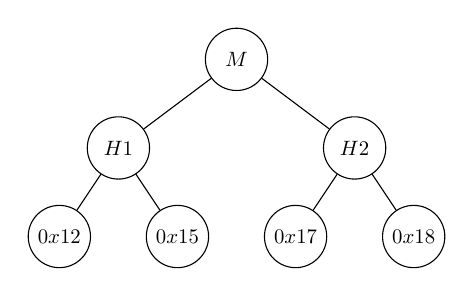
\begin{tikzpicture}[scale=0.75,node distance=20mm, 
  every node/.style={transform shape},
  level/.style={sibling distance=40mm/#1}
]

\tikzstyle{vertex}=[draw,circle,minimum size=30pt,inner sep=0pt]

\node [vertex] (r1){$M$}
  child {
    node [vertex] {$H1$}
    child {
      node [vertex] {$0x12$}
    }
    child {
      node [vertex] {$0x15$}
    }
  }
  child {
    node [vertex] {$H2$}
    child {
      node [vertex] {$0x17$}
    }
    child {
      node [vertex] {$0x18$}
    }
  };
\end{tikzpicture}  
\caption{Transactions in Merkle trees are in ascending order\label{fig:BloomFalsePositive}}
\end{figure}  
\end{example}

\subsection{Transaction Aggregation}
\label{Design:TransactionAggregation}

Transaction aggregation is a way of keeping the size of the ledger small, that is, validators only store transactions not older than a predefined number of blocks, denoted as aggregation length $length_{ag}$. A special type of transaction called \textit{Aggregation Transaction (AggTx)} is created by summing up transferred amounts either by sender or by receiver.

\begin{figure}[hbt]
\centering
\begin{subfigure}[b]{0.9\textwidth}
  \centering
  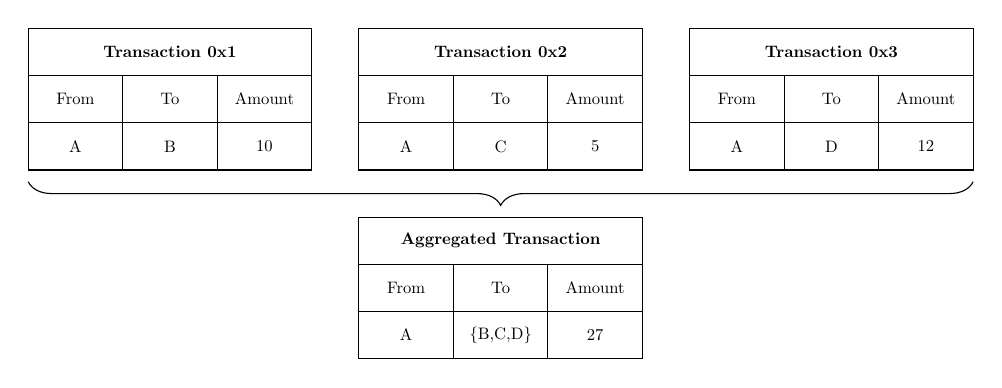
\begin{tikzpicture}[scale=0.6, every node/.style={transform shape}]

  % ***************** Agg Tx ***************** 
  
  \draw (7,0) rectangle (13,3);
  \draw (7,2) -- (13,2);
  \draw (9,0) -- (9,2);
  \draw (11,0) -- (11,2);
  \draw (7,1) -- (13,1);
  
  \node at (10,2.5) {\bfseries{Aggregated Transaction}};
  \node at (8,1.5) {From};
  \node at (8,0.5) {A};
  \node at (10,1.5) {To};
  \node at (10,0.5) {\{B,C,D\}};
  \node at (12,1.5) {Amount};
  \node at (12,0.5) {27};
  
  % ***************** TX 1 ***************** 
  
  \draw (0,4) rectangle (6,7);
  \draw (0,6) -- (6,6);
  \draw (2,4) -- (2,6);
  \draw (4,4) -- (4,6);
  \draw (0,5) -- (6,5);
  
  \node at (3,6.5) {\bfseries{Transaction 0x1}};
  \node at (1,5.5) {From};
  \node at (1,4.5) {A};
  \node at (3,5.5) {To};
  \node at (3,4.5) {B};
  \node at (5,5.5) {Amount};
  \node at (5,4.5) {10};
  
  % ***************** TX 2 ***************** 
  
  \draw (7,4) rectangle (13,7);
  \draw (7,6) -- (13,6);
  \draw (9,4) -- (9,6);
  \draw (11,4) -- (11,6);
  \draw (7,5) -- (13,5);
  
  \node at (10,6.5) {\bfseries{Transaction 0x2}};
  \node at (8,5.5) {From};
  \node at (8,4.5) {A};
  \node at (10,5.5) {To};
  \node at (10,4.5) {C};
  \node at (12,5.5) {Amount};
  \node at (12,4.5) {5};
  
  % ***************** TX 2 ***************** 
  
  \draw (14,4) rectangle (20,7);
  \draw (14,6) -- (20,6);
  \draw (16,4) -- (16,6);
  \draw (18,4) -- (18,6);
  \draw (14,5) -- (20,5);
  
  \node at (17,6.5) {\bfseries{Transaction 0x3}};
  \node at (15,5.5) {From};
  \node at (15,4.5) {A};
  \node at (17,5.5) {To};
  \node at (17,4.5) {D};
  \node at (19,5.5) {Amount};
  \node at (19,4.5) {12};
  
  % ***************** BRACE ***************** 
  
  \draw[decoration={brace,mirror,amplitude=3mm},decorate]
    (0,3.75) -- node[right=12pt] {} (20,3.75);
  
  \end{tikzpicture}
  \caption{Transaction aggregation by sender.\label{fig:TxAggBySender}}
\end{subfigure}
\par\bigskip
\begin{subfigure}[b]{0.9\textwidth}
  \centering
  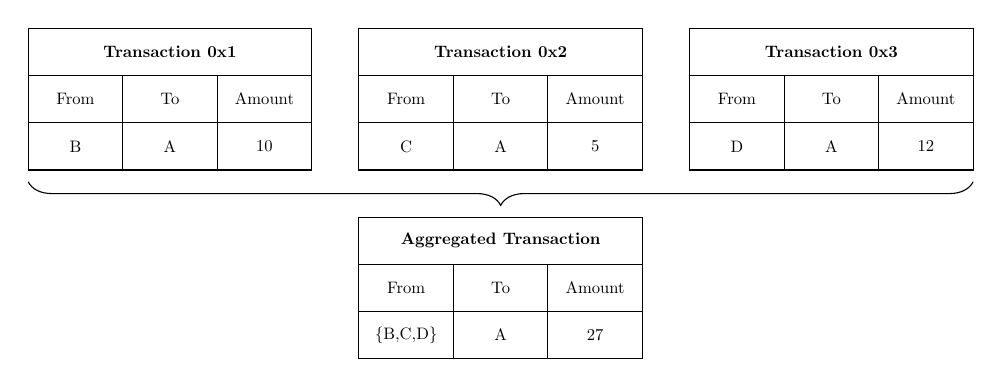
\begin{tikzpicture}[scale=0.6, every node/.style={transform shape}]
  % ***************** Agg Tx ***************** 
  
  \draw (7,0) rectangle (13,3);
  \draw (7,2) -- (13,2);
  \draw (9,0) -- (9,2);
  \draw (11,0) -- (11,2);
  \draw (7,1) -- (13,1);
  
  \node at (10,2.5) {\bfseries{Aggregated Transaction}};
  \node at (8,1.5) {From};
  \node at (8,0.5) {\{B,C,D\}};
  \node at (10,1.5) {To};
  \node at (10,0.5) {A};
  \node at (12,1.5) {Amount};
  \node at (12,0.5) {27};
  
  % ***************** TX 1 ***************** 
  
  \draw (0,4) rectangle (6,7);
  \draw (0,6) -- (6,6);
  \draw (2,4) -- (2,6);
  \draw (4,4) -- (4,6);
  \draw (0,5) -- (6,5);
  
  \node at (3,6.5) {\bfseries{Transaction 0x1}};
  \node at (1,5.5) {From};
  \node at (1,4.5) {B};
  \node at (3,5.5) {To};
  \node at (3,4.5) {A};
  \node at (5,5.5) {Amount};
  \node at (5,4.5) {10};
  
  % ***************** TX 2 ***************** 
  
  \draw (7,4) rectangle (13,7);
  \draw (7,6) -- (13,6);
  \draw (9,4) -- (9,6);
  \draw (11,4) -- (11,6);
  \draw (7,5) -- (13,5);
  
  \node at (10,6.5) {\bfseries{Transaction 0x2}};
  \node at (8,5.5) {From};
  \node at (8,4.5) {C};
  \node at (10,5.5) {To};
  \node at (10,4.5) {A};
  \node at (12,5.5) {Amount};
  \node at (12,4.5) {5};
  
  % ***************** TX 2 ***************** 
  
  \draw (14,4) rectangle (20,7);
  \draw (14,6) -- (20,6);
  \draw (16,4) -- (16,6);
  \draw (18,4) -- (18,6);
  \draw (14,5) -- (20,5);
  
  \node at (17,6.5) {\bfseries{Transaction 0x3}};
  \node at (15,5.5) {From};
  \node at (15,4.5) {D};
  \node at (17,5.5) {To};
  \node at (17,4.5) {A};
  \node at (19,5.5) {Amount};
  \node at (19,4.5) {12};
  
  % ***************** BRACE ***************** 
  
  \draw[decoration={brace,mirror,amplitude=3mm},decorate]
    (0,3.75) -- node[right=12pt] {} (20,3.75);
  
  \end{tikzpicture}
  \caption{Transaction aggregation by receiver.\label{fig:TxAggByReceiver}}
\end{subfigure}
\caption{Transaction aggregation types}
\end{figure}

In transaction aggregation by sender, transactions sent \textit{from} a particular user are summed up, shown in Figure \ref{fig:TxAggBySender}. On the contrary, in transaction aggregation by receiver, transactions sent \textit{to} a particular user are summed up, shown in Figure \ref{fig:TxAggByReceiver}. Furthermore, we distinguish between transaction aggregation performed by an aggregator or by a leader.

Firstly, transaction aggregation is performed by validators with the role \textit{aggregator}. An aggregator is elected per block height and per shard in the same way a leader is elected with the exception that the \textit{Role} property of Equation \ref{eq:PoSCondition} must be set to $"A"$. In rare cases, there can be zero or more aggregators per block height. If more than one validator fulfills the PoS condition \ref{eq:PoSCondition}, the validator who has the lowest value below \textit{Target} becomes an aggregator. Also note that an elected aggregator is not assigned to a random shard. An aggregator only aggregates transactions of the shard they are assigned to, because block bodies containing transactions with self-contained proofs are only stored by validators of the shard they are assigned.

After becoming an aggregator, transactions from previous blocks are aggregated by sender or receiver. Aggregated transactions are then filled into a special type of block called \textit{aggregation block}. An aggregation block of shard $s$ at block height $h$ serves as a proposal to a validator who becomes a leader of shard $s$ at block height $h + 1$. Informally, the following algorithm is performed by each aggregator at block height $h$:
\begin{enumerate}
  \item Create an empty aggregation block.
  \item Pick transactions in two ways:
    \begin{enumerate}
      \item For each shard block or aggregation block $b$, where $Height(b) \leq h - 1$, pick  transactions where each sender or receiver appears at least twice and where $Aggregated = false$. Note that $FundsTx$ as well as $AggTx$ can be aggregated.
      \item For each shard or aggregation block $b$, where $h - Height(b) \geq length_{ag}$, pick all transactions which have not been aggregated yet, i.e., where $Aggregated = false$.
    \end{enumerate}
  \item Sum up the amount of coins that have been sent or received, generate the transaction hash, create the aggregated transaction and add it to the aggregation block. Set $Aggregated \leftarrow true$ to transactions in the block they were picked from.
\end{enumerate}

Secondly, transaction aggregation is performed by validators with the role \textit{leader}. When a leader creating a block picks transaction from the local transaction pool, transactions of the same sender are aggregated to a single aggregated transaction. This task is crucial in order to prevent fraudulent proofs, evaluated in Section \ref{Eval:SecurityConsiderations}. A leader is also responsible for the verification at height $h$ of an aggregation block that has been proposed at block height $h - 1$. The verification process is performed in the same fashion as Bloom filter checks of self-contained proofs.

\subsection{Block Height Synchronisation}
\label{Design:BlockHeightSync}

The leader assignment process described in Section \ref{Design:LeaderAssignment} does not guarantee to have one leader per shard. As a result, a shard could have no leader at one block height resulting in a divergence of block heights among different shardchains. For this reason, the block height of shardchains must be synchronized with each other to ensure equally growing chains of blocks.

\begin{figure}[hbt]
  \centering
  \captionsetup{justification=centering}
  \begin{subfigure}[b]{0.45\textwidth}
    \centering
    \begin{tikzpicture}
        \tikzset{node style/.style={state,node distance=7mm,minimum width=3mm,minimum height=3mm,rectangle}}
    
        \node[node style]   (sb_2-1)  {};
        \node[node style, above=of sb_2-1]  (sb_1-1)  {};
        \node[node style, below=of sb_2-1]  (sb_3-1)  {};
        \node[node style, right=of sb_2-1]  (sb_2-2) {};
        \node[node style, above=of sb_2-2]  (sb_1-2) {};
        \node[node style, below=of sb_2-2]  (sb_3-2) {};
        \node[node style, right=of sb_3-2]  (sb_3-3) {};
        \node[node style, right=of sb_3-3]  (sb_3-4) {};
        \node[node style, right=of sb_2-2] (sb_2-3)  {};
        \node[node style, right=of sb_1-2] (sb_1-3)  {};
        \node[node style, right=of sb_1-3] (sb_1-4)  {};
        \node[node style, right=of sb_1-4] (sb_1-5)  {};
    
    \draw[>=latex,
          auto=left,
          every loop]
         (sb_1-2)  edge node {}   (sb_1-1)
         (sb_2-2)  edge node {}   (sb_2-1)
         (sb_3-2)  edge node {}   (sb_3-1)
         (sb_1-3)  edge node {}   (sb_1-2)
         (sb_1-4)  edge node {}   (sb_1-3)
         (sb_1-5)  edge node {}   (sb_1-4)
         (sb_2-3) edge node {}   (sb_2-2)
         (sb_3-3) edge node {}   (sb_3-2)
         (sb_3-4) edge node {}   (sb_3-3); 
    \end{tikzpicture}
    \caption{Without Synchronisation}
  \end{subfigure}
  ~
  \begin{subfigure}[b]{0.45\textwidth}
    \centering
    \begin{tikzpicture}
        \tikzset{node style/.style={state,node distance=7mm,minimum width=3mm,minimum height=3mm,rectangle}}
    
        \node[node style]   (sb_2-1)  {};
        \node[node style, above=of sb_2-1]  (sb_1-1)  {};
        \node[node style, below=of sb_2-1]  (sb_3-1)  {};
        \node[node style, right=of sb_2-1]  (sb_2-2) {};
        \node[node style, above=of sb_2-2]  (sb_1-2) {};
        \node[node style, below=of sb_2-2]  (sb_3-2) {};
        \node[node style, right=of sb_3-2]  (sb_3-3) {};
        \node[node style, right=of sb_3-3]  (sb_3-4) {};
        \node[node style, right=of sb_2-2] (sb_2-3)  {};
        \node[node style, right=of sb_2-3] (sb_2-4)  {};
        \node[node style, right=of sb_1-2] (sb_1-3)  {};
        \node[node style, right=of sb_1-3] (sb_1-4)  {};
    
    \draw[>=latex,
          auto=left,
          every loop]
         (sb_1-2)  edge node {}   (sb_1-1)
         (sb_2-2)  edge node {}   (sb_2-1)
         (sb_3-2)  edge node {}   (sb_3-1)
         (sb_1-3)  edge node {}   (sb_1-2)
         (sb_2-3) edge node {}   (sb_2-2)
         (sb_3-3) edge node {}   (sb_3-2)
         (sb_1-4)  edge node {}   (sb_1-3)
         (sb_2-4) edge node {}   (sb_2-3)
         (sb_3-4) edge node {}   (sb_3-3); 
         
    \draw[thin,double,<->,shorten >=4pt,shorten <=4pt,>=stealth,dotted]
         (sb_1-1)   edge node {}   (sb_2-1)
         (sb_2-1)   edge node {}   (sb_3-1)
         (sb_1-2)   edge node {}   (sb_2-2)
         (sb_2-2)   edge node {}   (sb_3-2)
         (sb_1-3)   edge node {}   (sb_2-3)
         (sb_2-3)   edge node {}   (sb_3-3)
         (sb_1-4)   edge node {}   (sb_2-4)
         (sb_2-4)   edge node {}   (sb_3-4);       
         
    \end{tikzpicture}
    \caption{With Synchronisation}
  \end{subfigure}
  \caption{Shardchains could diverge during due to network latency or other reasons resulting in different block heights.}
  \label{fig:shard_divergence}
\end{figure}

Validators receive blocks and have to perform at least one comparison operation per block in order to decide whether the block belongs to their shard or not. Hence, they can keep track of the number of blocks received at block height $h$. If the number equals to \textit{NofShards}, validators can be certain that each shardchain of the network grows equally at the same pace. Informally, the following algorithm is performed by each validator $v$ upon receiving block $b$:
\begin{enumerate}
  \item The validator checks if the block has already been processed by using the hash of the block and comparing it with the local database. If the block has not been processed yet, continue. Otherwise, the block has already been processed or deemed invalid and the algorithm stops.
  \item If $Height(b) = h$, where $Height$ is a function that returns the height of block, continue. Otherwise, the block does not belong to the current block height the algorithm stops.
  \item Where \textit{ShardOfBlock} is a function that returns the shard identifier for which a block was created for, and where \textit{ShardOfValidator} is a function that returns the shard identifier the validator belongs to, 
    \begin{enumerate}
      \item if $ShardOfBlock(b) = ShardOfValidator(v)$, locally store the block header and block body. For each transaction hash included in the block, the validator queries the transaction from the local transaction pool and deletes it, otherwise,
      \item if $ShardOfBlock(b) \neq ShardOfValidator(v)$, locally store only the block header.
    \end{enumerate}
    In either case, increment $ReceivedBlocks$ by one, where $ReceivedBlocks$ keeps track of the number of received blocks for block height $h$.
  \item Check the self-contained proof. If all Merkle proofs of the SCP are valid, redistribute the block immediately. Otherwise, stop the algorithm.
  \item If $ReceivedBlocks = NofShards$, set $ReceivedBlocks \leftarrow 0$ and start the leader election process, as explained in Section \ref{Design:LeaderElection}. Otherwise, repeat algorithm on arrival of the next block.
\end{enumerate}

\section{Epoch Finality}
\label{Design:Finality}

An epoch finishes after a predefined number of blocks, called \textit{epoch length}, denoted $length_{ep}$. As pointed out in Section \ref{Design:BlockHeightSync}, shardchains can grow in a non-deterministic way if two or more leaders are assigned to the same shard, but since shardchains are synchronized among each other, the finalization of an epoch is guaranteed to end almost at the same time.

Once $length_{ep}$ is reached, validators agree on an epoch block. This special type of block only serves as checkpoint. The network is then repartitioned based on the number of users $NofUsers$. An epoch block is not distributed because it is non-interactively created by every validator in the network. Each validator is able to derive the same hash based on previous blocks.


